\documentclass[american]{cv-class}
\usepackage{afterpage}
\usepackage{hyperref}
\usepackage{color}
\usepackage{xcolor}
\usepackage[raggedrightboxes]{ragged2e}
\addbibresource{ref.bib}

\hypersetup{
    colorlinks=true,
    linkcolor=blue
}

\RequirePackage{xcolor}
\definecolor{blue}{HTML}{0395DE}

\begin{document}
\header{Carlos Eduardo}{Orozco}
{Senior Java Analyst/Developer - Solution Architect }

\vspace{1.15cm}
\fcolorbox{white}{gray}{\parbox{\dimexpr\textwidth-2\fboxsep-2\fboxrule}{%
	.....
}}

\begin{aside}
	
\includegraphics[scale=0.10]{img/indice.jpeg}
	~
	\vspace{0.35cm}
	\section{Info/Contact}
	\textbf{Age:} 26 \\
	\textbf{Civil Status:} Single \\
	\textbf{Address:} Cra 51D 67A16 \\
	\textbf{Location:} Medellín, CO \\
	\textbf{Contact/Email:}\\ \href{https://bit.ly/3ls6eXV}{\raisebox{-0.35ex}{
\includegraphics[scale=0.06]{img/whatsapp-logo.jpg}}/+573116345180}\\
	\href{https://join.skype.com/invite/GVNxPbWtJxdc}{\raisebox{-0.35ex}{
\includegraphics[scale=0.11]{img/skype-logo.png}}/carlos.orozco22}\\
	\href{mailto:carlos940807@gmail.com}{\raisebox{-0.35ex}{
\includegraphics[scale=0.009]{img/gmail-logo.png}}/carlos940807}
	~
	\section{Work Contact}
	\href{https://linkedin.com/in/corozco9408}{\raisebox{-0.35ex}{
\includegraphics[scale=0.3]{img/linkedin-logo.png}}/in/corozco9408}
	\href{https://www.researchgate.net/profile/Carlos_Orozco29}{\raisebox{-0.35ex}{
\includegraphics[scale=0.05]{img/researchgate-logo.png}}/carlos.orozco29}	\href{https://orcid.org/0000-0003-2615-3294}{\raisebox{-0.35ex}{
\includegraphics[scale=0.7]{img/orcid-logo.png}}/0000-0003-2615-3294}
	~ 
	\section{Academic Contact}
	\href{mailto:carlosorozco@unicauca.edu.co}{\raisebox{-0.35ex}{
\includegraphics[scale=0.05]{img/unicauca-logo.png}}/carlosorozco} 	~
	\href{mailto:carlose.orozco@udea.edu.co}{\raisebox{-0.35ex}{
\includegraphics[scale=0.05]{img/udea-logo.png}}/carlose.orozco}
	~
	\section{Languages}
	\asidelist{\textbf{Spanish}}
	{
\includegraphics[scale=0.40]{img/5stars.png}}
	\asidelist{\textbf{English}}
	{
\includegraphics[scale=0.40]{img/4stars.png}}
	~
	\section{FrontEnd}
	\asidelist{\textbf{Angular 4+}}
	{
\includegraphics[scale=0.40]{img/5stars.png}}
	\asidelist{\textbf{Ionic}}
	{
\includegraphics[scale=0.40]{img/5stars.png}}
	~
	\section{BackEnd}
	\asidelist{\textbf{Java EE}}
	{
\includegraphics[scale=0.40]{img/5stars.png}}
	\asidelist{\textbf{Python 3.x}}
	{
\includegraphics[scale=0.40]{img/5stars.png}}
	\asidelist{\textbf{C\#}}
	{
\includegraphics[scale=0.40]{img/4stars.png}}
	\asidelist{\textbf{REST/SOAP}}
	{
\includegraphics[scale=0.40]{img/5stars.png}}
	~
	\section{Databases}
	\asidelist{\textbf{Oracle}}
	{
\includegraphics[scale=0.40]{img/5stars.png}}
	\asidelist{\textbf{MySql}}
	{
\includegraphics[scale=0.40]{img/5stars.png}}
	\asidelist{\textbf{PostgreSql}}
	{
\includegraphics[scale=0.40]{img/5stars.png}}
	
\end{aside}


\justifying
	\begin{small}
		\textit{
			I'm a system engineer with experience on backend develop. My main skills are business analysis in health and e-commerce areas, work as java Architect, senior Java analyst/Developer and Semi-Senior Python Developer. Currently, I work as a technical leader, senior Java developer/architect and consultant for the definition and description of software configuration management process (SCM). Further, i do research work on Software Configuration Management, Process improvement, DevOps, Software architecture best practices and quality ensurance.
		}
	\end{small}

\section{Experience}
\begin{entrylist}
	~ 
    \entry
	{Dec. 19 - Now}
	{Solution Architect}
	{DAWSIN SAS, Popayán, CO}
	{\justifying Perform the validation and monitoring of the architecture
	of new IT solutions developed by the organization to ensure its integrity and scalability over time.}
	~ 
    \entry
	{Mar. 17 - Now}
	{Freelance consultant}
	{Medellín and Popayán, CO}
	{\justifying Consulting on issues related to best practices for the development of JAVA solutions, software architecture, process improvement and software configuration management assurance.}
	~ 
    \entry
	{Oct. 19 - Now}
	{Senior Developer}
	{\href{https://tecso.coop/}{ \raisebox{-1.5ex}{
\includegraphics[scale=0.04]{img/tecso-logo.jpg}Tecso Ltda, Medellín, CO}}}
	{\justifying Carry out the implementation of assignments associated with the backend solutions for specific clients in the financial sector (web services, database, definition of routes and communication channels, development of new requirements and new initiatives)}
	~ 
    \entry
	{Nov. 18 - Oct. 19}
	{Software Architect}
	{\href{http://www.serviciosenweb.com/}{ \raisebox{-1.5ex}{
\includegraphics[scale=0.09]{img/sew-logo.jpg}Servicios en Web, Medellín, CO}}}
	{\justifying Carry out the definition, planning, development and analysis of technical and functional evaluations of the product developed by the company to ensure that quality standards and good practices are met during software development.}
	~ 
    \entry
	{Aug. 18 - Nov. 18}
	{Analyst/Developer}
	{\href{http://www.serviciosenweb.com/}{ \raisebox{-1.5ex}{
\includegraphics[scale=0.09]{img/sew-logo.jpg}Servicios en Web, Medellín, CO}}}
	{\justifying Perform tasks related to the analysis, development and implementation of solutions focused on products on e-commerce area.}
	~ 
    \entry
	{Jul. 16 - Jul. 18}
	{Fullstack Developer}
	{\href{https://sitis.com.co/}{ \raisebox{-1.5ex}{
\includegraphics[scale=0.05]{img/sitis-logo.png} SITIS SAS, Popayán, CO}}}
	{\justifying Development of IT solutions for the organization using specific technologies (JAVA EE, Primefaces, angular 6x, JPA, Hibernate, Oracle DB).}
	~ 
    \entry
	{Mar. 13 - Apr 15}
	{Software developer}
	{DAWSIN SAS, Popayán, CO}
	{\justifying Provide support in the design, analysis, development, testing and deployment process of the products developed by the organization.}
\end{entrylist}

\section{Recognitions and awards}
\begin{entrylist}
	\entry
	{Nov. 16}
	{Recognition for outstanding work}
	{\href{https://sitis.com.co/}{ \raisebox{-1.5ex}{
\includegraphics[scale=0.05]{img/sitis-logo.png} SITIS SAS, Popayán, CO}}}
	{\href{https://bit.ly/38BDFnj}{\raisebox{-0.35ex}{
\includegraphics[scale=0.025]{img/certificado-logo.png}}{\addfontfeature{Color=blue}{\textit{View certificate}}}}
	}
	
	\entry
	{Dic. 17}
	{Best Employee Award}
	{\href{https://sitis.com.co/}{ \raisebox{-1.5ex}{
\includegraphics[scale=0.05]{img/sitis-logo.png} SITIS SAS, Popayán, CO}}}
	{\href{https://bit.ly/3pnroJ3}{\raisebox{-0.35ex}{
\includegraphics[scale=0.025]{img/certificado-logo.png}}{\addfontfeature{Color=blue}{\textit{View certificate}}}}
	}
	
\end{entrylist}

\newpage

\begin{aside}
	\section{SO}
	\asidelist{\textbf{Linux}}
	{
\includegraphics[scale=0.40]{img/5stars.png}}
	\asidelist{\textbf{Windows}}
	{
\includegraphics[scale=0.40]{img/5stars.png}}
	~
	\section{Methodologies and frameworks } \\
	\asidelist{\textbf{SCRUM}}
	{
\includegraphics[scale=0.40]{img/5stars.png}}
	\asidelist{\textbf{LEAN}}
	{
\includegraphics[scale=0.40]{img/5stars.png}}
	\asidelist{\textbf{XP}}
	{
\includegraphics[scale=0.40]{img/5stars.png}}
	\asidelist{\textbf{DevOps}}
	{
\includegraphics[scale=0.40]{img/5stars.png}}
	\asidelist{\textbf{TDD}}
	{
\includegraphics[scale=0.40]{img/5stars.png}}
	\asidelist{\textbf{SCM}}
	{
\includegraphics[scale=0.40]{img/5stars.png}}
	    
	~
	\section{Places lived}
	\\
	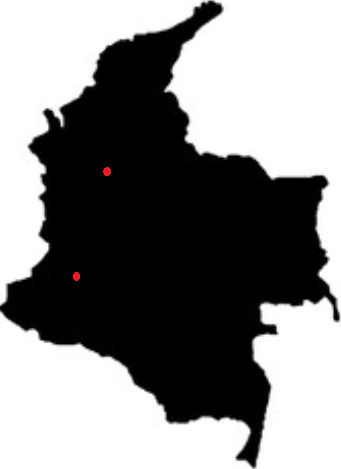
\includegraphics[scale=0.42]{img/colombia-logo.png}
	~
\end{aside}

\section{Education}
\begin{entrylist}
	\entry
	{Aug. 20 - Now}
	{Computer Science PhD}
	{{
\includegraphics[scale=0.05]{img/unicauca-logo.png}} Universidad del Cauca, CO} 
	{\justifying Doctoral studies focused on software process improvement and quality assurance through agile approaches. Currently doing research work related to evaluation models for DevOps supported in inference techniques with artificial intelligence.}
	
	\entry
	{Aug. 20 - Now}
	{Computing Master Degree (MSc)}
	{ \raisebox{-1.5ex}{
\includegraphics[scale=0.05]{img/unicauca-logo.png} Universidad del Cauca, CO}}
	{\justifying Postgraduate studies focused directly on the improvement of processes and evaluation of DevOps in software development companies.}
	
	\entry
	{Aug. 18 - Now}
	{Astronomy Degree}
	{ \raisebox{-1.5ex}{
\includegraphics[scale=0.05]{img/udea-logo.png}Universidad de Antioquia, CO}}
	{\justifying Currently studying the curriculum to obtain the title of Astronomer.}
	
	\entry
	{Aug. 11 - Mar. 17}
	{System Engineering Degree}
	{ \raisebox{-1.5ex}{
\includegraphics[scale=0.05]{img/unicauca-logo.png} Universidad del Cauca, CO}}
	{\justifying Systems engineering graduate professional with the ability to identify problems and propose software solutions in accordance with their environment.

	\href{https://bit.ly/3ppF1aU}{\raisebox{-0.35ex}{
\includegraphics[scale=0.025]{img/certificado-logo.png}}{\addfontfeature{Color=blue}{ \textit{Degree certificate}}}}
   
	\href{https://bit.ly/38BkZ7l}{\raisebox{-0.35ex}{
\includegraphics[scale=0.011]{img/diploma-logo.png}}{\addfontfeature{Color=blue}{    \textit{Diploma}}}}
	}
	
	\entry
	{Jan. 04 - Dec. 10}
	{Software Development Technical Bachelor}
	{ \raisebox{-1.5ex}{
\includegraphics[scale=0.007]{img/industrial-logo.png} Instituto Técnico Industrial, CO}}
	{Bachelor degree with emphasys on software development.}
	
	\entry
	{Jan. 00 - Dec. 04}
	{Basic primary degree.}
	{ \raisebox{-1.5ex}{
\includegraphics[scale=0.007]{img/industrial-logo.png} Instituto Técnico Industrial, CO}}
	{Basic primary degree}
\end{entrylist}

\section{Projects}
\begin{entrylist}
	\entry
	{Now}
	{BANCOLOMBIA PERSON APP}
	{\href{https://www.grupobancolombia.com/personas}{ \raisebox{-1.5ex}{
\includegraphics[scale=0.05]{img/bancolombia-logo.png} Bancolombia, Medellín, CO}}}
	{\justifying External provider that performs tasks related toImplementation of services, communication channels, platform, database and backend for initiatives related to new Bancolombia projects.}
	
	\entry
	{Nov. 17}
	{AUDAMEDIC – AUDATEX México}
	{\href{https://sitis.com.co/}{ \raisebox{-1.5ex}{
\includegraphics[scale=0.05]{img/sitis-logo.png} SITIS SAS, Popayán, CO}}}
	{\justifying Development of an assurance system for Audatex México in
	Java EE Backend and Primefaces Frontend thecnologies.}
	  
	\entry
	{Sep. 15}
	{SMAC-JPA}
	{ \raisebox{-1.5ex}{DAWSIN SAS, Popayán, CO}}
	{\justifying Assurance System for AIC-EPSI. Use of Java EE with REST Api for the Backend and Angular 5 Frontend.}
	
	\entry
	{Aug. 14}
	{CENSO WEB}
	{ \raisebox{-1.5ex}{DAWSIN SAS, Popayán, CO}}
	{\justifying PHP system to capture the population census of the indigenous council of Pitayó-Cauca.}
	
	\entry
	{Jan. 14}
	{VENTAS MOVIL}
	{ \raisebox{-1.5ex}{DAWSIN SAS, Popayán, CO}}
	{\justifying Sell system development in JAVA Web and Android, sales application TAT.}
	
	\entry
	{May. 13}
	{NETCOM}
	{ \raisebox{-1.5ex}{DAWSIN SAS, Popayán, CO}}
	{\justifying Development and validation of architecture in JAVA EE for
	all tasks related to the backend using the implementation of generic query models.}
	
\end{entrylist}

\newpage

\section{Certifications}
\begin{entrylist}
	\entry
	{2020}
	{Desarrollo Ágil de software}
	{\raisebox{-1.5ex}{
\includegraphics[scale=0.3]{img/linkedin-logo.png}}}{\href{https://bit.ly/3njvqk1}{\raisebox{-0.35ex}{
\includegraphics[scale=0.025]{img/certificado-logo.png}}{\addfontfeature{Color=blue}{\textit{View certificate}}}}}
	
	\entry
	{2020}
	{Introduction to Astrophysics}
	{\raisebox{-1.5ex}{
\includegraphics[scale=0.2]{img/edx-logo.png}}}{\href{https://bit.ly/32FJIUe}{\raisebox{-0.35ex}{\includegraphics[scale=0.025]{img/certificado-logo.png}}{\addfontfeature{Color=blue}{\textit{View certificate}}}}}
	
	\entry
	{2020}
	{Java EE: Design Patterns and Architecture}
	{ \raisebox{-1.5ex}{\includegraphics[scale=0.3]{img/linkedin-logo.png}}}{\href{https://bit.ly/3pyEgwi}{\raisebox{-0.35ex}{\includegraphics[scale=0.025]{img/certificado-logo.png}}{\addfontfeature{Color=blue}{\textit{View certificate}}}}}

	\entry
	{2020}
	{Java avanzado, buenas prácticas}
	{\raisebox{-1.5ex}{\includegraphics[scale=0.3]{img/linkedin-logo.png}}}{\href{https://bit.ly/35uFhO1}{\raisebox{-0.35ex}{\includegraphics[scale=0.025]{img/certificado-logo.png}}{\addfontfeature{Color=blue}{\textit{View certificate}}}}}
	
	\entry
	{2020}
	{Python para data scientist avanzado}
	{ \raisebox{-1.5ex}{\includegraphics[scale=0.3]{img/linkedin-logo.png}}}{\href{https://bit.ly/3pqLZw7}{\raisebox{-0.35ex}{\includegraphics[scale=0.025]{img/certificado-logo.png}}{\addfontfeature{Color=blue}{\textit{View certificate}}}}}
	
	\entry
	{2020}
	{Contribution to observation of near-Earth objects}
	{ \raisebox{-1.5ex}{\includegraphics[scale=0.07]{img/nasa-logo.png}}}
	{\href{https://bit.ly/3knGoD7}{\raisebox{-0.35ex}{\includegraphics[scale=0.025]{img/certificado-logo.png}}{\addfontfeature{Color=blue}{\textit{View certificate}}}}}
	
	\entry
	{2019}
	{Security Core Training}
	{ \raisebox{-1.5ex}{\includegraphics[scale=0.05]{img/sans-logo.png}}}{\href{https://bit.ly/3nfJBGP}{\raisebox{-0.35ex}{\includegraphics[scale=0.025]{img/certificado-logo.png}}{\addfontfeature{Color=blue}{\textit{View certificate}}}}}
	\entry
	{2016}
	{Scrum Fundamentals Certified Credential}
	{ \raisebox{-1.5ex}{\includegraphics[scale=0.035]{img/scrumstudy-logo.jpg}}}{\href{https://bit.ly/38PJnCr}{\raisebox{-0.35ex}{\includegraphics[scale=0.025]{img/certificado-logo.png}}{\addfontfeature{Color=blue}{\textit{View certificate}}}}}
	
\end{entrylist}

\section{Publications and Conferences}
\begin{entrylist}
	\entry
	{2020}
	{Progresconfig: A SCM process}
	{ \raisebox{-1.5ex}{\includegraphics[scale=0.15]{img/risti-logo.png}}}
	{\justifying Article accepted on Revista Ibérica de Sistemas y Tecnologías de la Información (RISTI). Speaker of accepted article at: III Congreso Internacional de Sistemas Inteligentes y Nuevas Tecnologías: Tendencias Interdisciplinarias en Salud (COISINT 2020) \\
	{\href{https://bit.ly/3eUN9Ly}{\raisebox{-0.35ex}{\includegraphics[scale=0.025]{img/certificado-logo.png}}{\addfontfeature{Color=blue}{\textit{View certificate}}}}}
	}
	\entry
	{2020}
	{SCMOnto: A SCM Ontology}
	{ \raisebox{-1.5ex}{\includegraphics[scale=0.15]{img/risti-logo.png}}}
	{\justifying Article accepted on Revista Ibérica de Sistemas y Tecnologías de la Información (RISTI). Speaker of accepted article at: XV Jornadas Iberoamericanas de Ingeniería de Software e Ingeniería del Conocimiento (JIISIC 2020) \\
	{\href{https://bit.ly/36BxP2W}{\raisebox{-0.35ex}{\includegraphics[scale=0.025]{img/certificado-logo.png}}{\addfontfeature{Color=blue}{\textit{View certificate}}}}}
	}
	
	\entry
	{2015}
	{II Jornada Iberoamericana de Interacción Humano Computador}
	{}
	{Assistant.
		    
	{\href{https://bit.ly/2UiQBGx}{\raisebox{-0.35ex}{\includegraphics[scale=0.025]{img/certificado-logo.png}}{\addfontfeature{Color=blue}{\textit{View certificate}}}}}
	}
\end{entrylist}

\newpage

\section{Volunteering Experience}
\begin{entrylist}
	  
	\entry
	{Jul. 18 - Now}
	{Monitor}
	{{\includegraphics[scale=0.05]{img/udea-logo.png}} Universidad de Antioquia, CO} 
	{\justifying Assist and guide first-semester students in areas related to exact sciences in fundamental concepts of algorithm and language-oriented programming.}
	  
	\entry
	{Sep. 18 - Mar. 20}
	{Thesis Co-Director}
	{{\includegraphics[scale=0.05]{img/unicauca-logo.png}} Universidad del Cauca, CO} 
	{\justifying Support and follow-up to degree projects of students of systems engineering at the University of Cauca on process improvement and software quality areas.}
	
	\entry
	{Aug. 15 - Dec 17}
	{Monitor}
	{{\includegraphics[scale=0.05]{img/unicauca-logo.png}} Universidad del Cauca, CO} 
	{\justifying Assist lower semester students in topics related to the development of web applications using business architectures. Application of best practices for software development on topics of: Continuous integration, code documentation source, unit tests, design patterns and good practices in object-oriented software development.}
	
\end{entrylist}


\section{References}
\begin{entrylist}
	  
	\entry
	{Academic}
	{PhD. MSc. Eng. César Pardo}
	{System Engineering} 
	{Phone: +573508479834, Popayán, CO.}
	
	\entry
	{Academic}
	{PhD. MSc. Eng. Fracisco Pino}
	{System Engineering} 
	{Phone: +573218942563, Popayán, CO.}
	
	\entry
	{Laboral}
	{Eng. Jorge Gomez}
	{System Engineering} 
	{Phone: +573153564186, Popayán, CO.}
	
	\entry
	{Laboral}
	{Lic. Felipe Salazar}
	{Bussiness Administrator} 
	{Phone: +573136066832, Cali, CO.}
	
	\entry
	{Personal}
	{Eng. Edward Orozco}
	{System Engineering} 
	{Phone: +573174281839, Popayán, CO.}
	
	\entry
	{Personal}
	{Lic. Rocio Orozco}
	{Master in Plastic Arts} 
	{Phone: +573156215575, Cali, CO.}
	
\end{entrylist}

\vspace{0.5cm}
\begin{center}
	\emph{For all legal purposes I certify that all
		the answers and information written down by me,
		in this resume are true (C.S.T.
	Art.62 num. 1st)}
\end{center}

\begin{flushright}
    	\emph{{\includegraphics[scale=0.55]{img/firma.JPG}}}
\end{flushright}
\begin{flushright}
	\emph{\textbf{CARLOS EDUARDO OROZCO GARCÉS}}
\end{flushright}
\begin{flushright}
	\emph{C.C. 1061772393. Popayán, CO}
\end{flushright}

\end{document}